\documentclass[11pt]{article}
\usepackage{amsmath, amssymb, amscd, amsthm, amsfonts}
\usepackage{graphicx}
\usepackage{hyperref}
\usepackage{acronym}
\usepackage{listings}
\usepackage[margin=2cm]{geometry}
\usepackage{endnotes}
\usepackage{tikz}
\usepackage{blindtext}
\usepackage{minipage-marginpar}
\usepackage{wrapfig}
% for pseudocode
\usepackage{algorithm}
\usepackage[noend]{algpseudocode}

% change language to german
\usepackage[utf8]{inputenc}
\usepackage[T1]{fontenc}
\usepackage[ngerman]{babel}
\usepackage{hyphenat}
% ---------

% for code style
\usepackage{xcolor}

\definecolor{codegreen}{rgb}{0,0.6,0}
\definecolor{codegray}{rgb}{0.5,0.5,0.5}
\definecolor{codepurple}{rgb}{0.58,0,0.82}
\definecolor{backcolour}{rgb}{0.95,0.95,0.92}

\lstset{ 
    language=C,
    backgroundcolor=\color{backcolour},   
    commentstyle=\color{codegreen},
    keywordstyle=\color{magenta},
    numberstyle=\tiny\color{codegray},
    stringstyle=\color{codepurple},
    basicstyle=\ttfamily\footnotesize,
    breakatwhitespace=false,         
    breaklines=true,                 
    keepspaces=true,                 
    numbers=left,       
    numbersep=5pt,                  
    showspaces=false,                
    showstringspaces=false,
    showtabs=false,                  
    tabsize=2,           % show the filename of files included with \lstinputlisting; also try caption instead of title
} 

% ----------------------

\usepackage{glossaries}

\oddsidemargin 0pt
\evensidemargin 0pt
\marginparwidth 40pt
\marginparsep 10pt
\topmargin -20pt
\headsep 10pt
\textheight 8.7in
\textwidth 6.65in
\linespread{1}

% for centering the title page
\usepackage{titling}
\renewcommand\maketitlehooka{\null\mbox{}\vfill}
\renewcommand\maketitlehookd{\vfill\null}

% usesul macros
\newcommand{\lstin}[1]{\lstinline[language=C]{#1}}
\newcommand{\cpl}{\textbf{C}$\;$}

% for footnotes
\renewcommand{\notesname}{Fußnoten}
\let\footnote=\endnote

% ------- glossary -------
% to build the glossary when changed run the build make_glossaries.cmd file first
\makeglossaries

% TODO: sources for definitions
\newglossaryentry{bm}
{
  name=Benchmark,
  description={Test für die Zeitkomplexität und Speicherkomplextät von Software},
}

\newglossaryentry{dt}
{
  name=Datenstruktur,
  description={Strukturen, die Daten effizient speichern und einen effizienten Zugriff auf diese erlauben \cite[S. VIII]{aad}},
  plural={Datenstrukturen}
}

\newglossaryentry{sc}
{
  name=Quelltext,
  description={Gesamtheit der Anweisungen eines Computerprogramms},
  plural={Quelltexte}
}

\newglossaryentry{wc}
{
  name={Worst Case},
  description={Konfiguration der Daten in einer Datenstruktur, bei der sie am schlechtesten arbeitet (z.B. besonders viel Zeit zur Datenverarbeitung benötigt oder besonders viel Speicher benötigt)},
  plural={Worst Cases}
}

\newglossaryentry{gns}
{
  name={Generic},
  description={TODO},
  plural={Generics}
}

\newglossaryentry{hp}
{
  name={Heap},
  description={TODO},
  plural={Heaps}
}

\newglossaryentry{sts}
{
  name={Struct},
  description={TODO},
  plural={Structs}
}

\newglossaryentry{uns}
{
  name={Union},
  description={TODO},
  plural={Unions}
}

\newglossaryentry{mc}
{
  name={Macro},
  description={TODO},
  plural={Macros}
}

\newglossaryentry{st}
{
  name={Stack},
  description={TODO},
  plural={Stacks}
}

\newglossaryentry{sof}
{
  name={Stackoverflow},
  description={TODO},
  plural={Stackoverflows}
}

\newglossaryentry{rec}
{
  name={Rekursion},
  description={Überbegriff für Programme oder Funktionen, die sich selbst aufrufen oder durch sich selbst definiert sind. \cite[S. 52]{aic} (z.B. \[
n! :=
  \begin{cases}
      n \cdot (n - 1)! ,& \text{wenn} \; n \neq 0\\
      1,              & \text{wenn} \; n = 0
  \end{cases}, \; n \in \mathbb{N}
\]
)},
  plural={Rekurionen}
}

\newglossaryentry{tv}
{
  name={Traversierung},
  description={TODO},
  plural={Traversierungen}
}

\newglossaryentry{psc}
{
  name={Pseudocode},
  description={TODO},
  plural={Pseudocodes}
}

\newglossaryentry{rcd}
{
  name={Rekursionstiefe},
  description={TODO},
}

\newglossaryentry{arr}
{
  name={Array},
  description={TODO},
  plural={Arrays}
}

\newglossaryentry{wch}
{
  name={Worst-Case-Höhe},
  description={TODO},
}
% ------- acronyms -------
\newacronym{rbt}{RBT}{Red Black Tree}
\newacronym{bt}{BT}{Binary Tree}


% ------- glossary -------

\title{\textbf{Seminararbeit Red-Black Trees}}
\author{Herr Yannik Höll}
\date{\today}

\begin{document}

\begin{titlingpage}
    \maketitle
\end{titlingpage}
\pagebreak

\tableofcontents
\pagebreak

\glsaddall
\printglossary
\pagebreak

\section{Einleitung}

% Einführungssätze

% Motivation der Datenstruktur
Eine Möglichkeit Daten so geordnet zu speichern sind so genannte Baumdatenstrukturen. Diese Speichern Werte geordnet nach einem bestimmten Schlüssel.
Eine sehr einfache Baumimplemntierung ist der \gls{bt} welcher jeweils nur 2 Abzweigungen pro Knoten besitzt (rigorose Baumdefinition in Kapitel \ref{def}).
Leider hat diese naiive Variante der Datenstruktur einige Probleme, welche vorallem beim Einfügen der Daten in geordneter Reigenfolge entstehen.
Um diese Probleme zu umgehen kann man die Algorithmen zum Einfügen und Entfernen neuer Datensätze so anpassen, dass die Baumstruktur performanter wird.
Ein möglicher besserer Ansatz sind die \glspl{rbt}.

% Inhalt der Arbeit
Diese Arbeit beschreibt wie sich \gls{rbt} von normalen \glspl{bt} unterscheiden. Es wird ausführlich beschrieben, wie normale \glspl{bt} funktionieren und wie man
ihre Algorithmen erweitert um \glspl{rbt} zu erhalten.
Dazu wurden jeweils beide \glspl{dt} in der Programmiersprache \cpl implementiert. Auf den jeweiligen \gls{sc} wird auch eingegangen um auf bestimmte Schwierigkeiten und Besonderheiten und den Implementierungen einzugehen.
Zudem werden die Ergenisse von \gls{bm} analysiert, welche zeigen sollen, dass \glspl{rbt} tatsächlich besser Laufzeiteigenschaften haben als
die Standimplementierung der \glspl{bt}.
Außerdem wird auf die Speicher- und Zeitkomplexität der beiden \glspl{dt} eingegangen und wie sich vorallem der \gls{rbt} im \gls{wc} verhält.

% TODO: Code Disclaimer shortned versions


\section{Definition Binary Tree \& Red Black Tree} \label{def}

\section{Implementierung}
Wie schon in den vorhergenden Kapiteln beschrieben, handelt es sich bei den Bäumen um eine generische Datenstruktur, in die der Nutzer beliebig Daten mit einem bestimmten Schlüssel einfügen kann.

Die Implementierung stellt deswegen 3 Funktionen bereit, mit denen man nach einem bestimmten Schlüssel im Baum suchen kann, man einen neuen Schlüssel zusammen mit einem Datensatz einfügen kann und man einen Schlüssel und den Datensatz wieder aus dem Baum löschen kann.

\subsection{Generics in C}
Bei der Implementierung in \cpl gab es dabei einige Schwierigkeiten, die man lösen musste. Es beginnt damit, dass \cpl keine objekt-orientierte Programmiersprache ist und keine eingebaute Möglichkeit für \glspl{gns} hat.
Nun kann man dieses Problem auf verschiedene Weisen lösen. Den Wert, der bei jedem Knoten des Baums gespeichert werden soll, lässt sich ganz simple aus Void-Pointer (\lstin{void*}) implementieren, sodass man die Daten beispielsweise auf dem \gls{hp} ablegen kann
und mithilfe eines Casts den Pointer der Daten (z.B. \lstin{int*}) zu \lstin{void*} umwandeln kann. Das erlaubt es, beliebige Datentypen und sogar \gls{sts} in den Baum einzufügen.
Diese Variante ist möglich, da die Nutzerdaten auf die Suche nach einem Knoten keinen Einfluss haben.

Anders ist es bei der Implementierung der Schlüssel. Hier muss sichergestellt sein, dass diese untereinander vergleichbar sind, sodass man die Suche, wie im Kapitel \ref{def} beschrieben, durchführen kann.
Man könnte Gebrauch von \glspl{uns} in \cpl machen, in denen man die numerischen Datentypen als mögliche Schlüssel anbietet.

\begin{lstlisting}[language=C]
union RBTreeKey {
  char c;
  short s;
  int i;
  long long l;
  float f;
  double d;
}
\end{lstlisting}

Zusätzlich müsste man dazu noch angeben, welchen Datentyp man in seinem Code nutzt (z.B. mithilfe einer \gls{mc}). Dieser Ansatz ist allerdings sehr unflexibel, weil man auf die Datentypen, die im \lstin{union RBTreeKey} vom Programmierer festgelegt sind, beschränkt ist.

Ein bessere Ansatz ist es, eine \gls{mc} zu definieren, die den Typen der Schlüssel definiert. Zusätzlich kann man noch eine 2. und 3. \gls{mc} definieren, die die Kleiner-Als- und Ist-Gleich-Operatoren definieren.
Das ermöglicht es beliebige Datentypen als Schlüssel zu verwenden (sogar \glspl{sts}), solange man die Vergleichsmacros definieren kann.

\begin{lstlisting}[language=C]
#define T int
#define TEQUAL(x, y) ((x) == (y))
#define TLESS(x, y) ((x) < (y))
\end{lstlisting}

Genau diese Implementierung wurde auch gewählt. Im Usercode müssen nur der Typ T und die Vergleichsoperationen TLESS und TEQUAL definiert werden. Einziger Nachteil ist, dass man im selben \gls{sc} nicht meherere verschidene Varianten von Schlüsseldatentypen nutzen kann.

\subsection{Knoten als Struct}
Wie schon in Kapitel \ref{def} beschrieben, sind Bäume nichts anders als ein 3-Tupel $(l, k, r)$.
$l$ und $r$ sind die Unterbäume und $k$ ist die Wurzel des Baumes (hier als $k$ bezeichnet wegen Schlüssel $\widehat{=}$ Key).
Jeder Knoten enthält somit seinen Schlüssel und eine Referenz auf den linken und rechten Unterbaum.
In \cpl wird der Baum nun als verkettete Liste von Knoten dargestellt
\footnote{Theoretisch gibt es auch eine Möglichkeit die Baumstruktur als \gls{arr} von Knoten darzustellen und bessere Cacheladezeiten zu bekommen.
Das größte Problem beim der Implementierung als verkettete Datenstruktur ist, dass die einzelnen Knoten stark verstreut im Heap abgespeichert sind und somit es zu vielen Cache Misses kommt. Diese Streuung kommt durch die Implementierung von \lstin{malloc} in der \cpl-Standart-Bibliothek zu stande ("The order and contiguity of storage allocated by successive calls to malloc() is unspecified." \cite{IEEEmalloc}). Das verlangsamt das Programm.
Man könnte als Array Implementierung eine spezielle Möglichkeit nutzen, Indizes für das Strukturieren des Arrays in Parent und Child zu nutzen.
Die Root würde den Index 0 erhalten. Die linken und rechten Kinder dann jeweils den Index $2 \cdot n + 1$ und $2 \cdot n + 2$ ($n$ ist der Index des Parents). So erhält jeder Knoten einen eindeutigen Index und es gibt eine eindeutige Parent-Child-Beziehung.
Leider ist der Red-Black-Tree kein vollständig balancierter Binary Tree, sodass es im Worst Case (Kapitel \ref{time}) passieren kann, dass sehr viel Speicher verschwendet wird, weil sehr viele Stellen im Array unbesetzt bleiben. Deswegen habe ich mich dagegen entschieden und habe die verkettete Variante der Datenstruktur implementiert.
}.
Im \lstin{struct Node} haben wir somit den generischen Schlüssel \lstin{T *key} und zugehörigen Wert \lstin{void *value}.
Zusätzlich speichern wir Pointer zum linken und rechten Child, welche die Wurzeln der entsprechenden Unterbäume sind. Zusätzlich wird auch noch ein Pointer zum Parent gespiechert,
da man diesen ziemlich oft in den Algorithmen zum Einfügen und Löschen von Knoten benötogt und man so den Quellcode etwas vereinfachen kann.

Natürlich gibt es im Knoten auch noch ein Feld, welches die Farbe des Knotens speichert. Diese ist später wichtig, weil sie von zum balancieren des Baumes benötigt wird.
Dieses findet während des Einfügens und Löschens neuer Knoten in den Baum statt. Die Werte für dieses Feld im \gls{sts} werden durch die \glspl{mc} \lstin{RB_TREE_RED} und \lstin{RB_TREE_BLACK} definiert.

Zusätzlich existiert ein weiter \gls{sts} für den Baum selbst, welcher allerdings nur als Handle für die Funktionen dient. Er speichert die Wurzel
und die Anzahl der eingefügten Knoten. Diese wird benötigt, damit man die \gls{wch} des Baums berechnen kann
\footnote{Die Worst-Case-Höhe wird für eine kleine Optimierung benötigt. Im Kapitel \ref{tr} wird beschrieben, wie man die Bäume traversiert.
Das ist normalerweise eine rekursive Operation, die ich jedoch iterativ implementiert habe. Dafür werden \glspl{st} benötigt, die sich dynamisch vergrößern, falls sie überlaufen würden.
Ich habe diese Stacks jedoch so implementiert, dass man sie mit einer initialen Größe erstellen kann. Die Worst-Case-Höhe des Baums gibt nun ungefähr die größte \gls{rcd} an, welche bei mir der größten Anzahl an Elementen auf dem Stack entspricht.
Somit kann ich dem Stack von Anfang an schon genug Platz geben, sodass er sich nicht so oft vergrößern muss, was mit einem Aufruf von \lstin{reallocarray()} verbunden.
Dabei wird ein großer Speicherbereich kopiert, was das Programm unnötig verlangsamt, wenn man zu oft mehr Speicher im Stack benötigt.
}.

\begin{lstlisting}[language=C]
#define RB_TREE_RED     1U
#define RB_TREE_BLACK   0U

struct Node;

struct Node {
    void *value;

    T *key;

    struct Node *left;
    struct Node *right;
    struct Node *parent;

    uint8_t color;
};

struct RBTree {
    struct Node *root;

    size_t node_count;
};
\end{lstlisting}

Zusätzlich existieren 2 Helfer-Funktionen, die jeweils eine Instanz von diesem \gls{sts} für den Nutzer erstellen und auch wieder freigeben. Der Baum wird durch die \lstin{create_tree} Funktion auf dem Heap abgespeichert und aus wird lediglich ein Pointer zu ihr ausgegeben.
Das Löschen des Baumes wird durch \lstin{free_tree} implementiert. Dieses ist auch auf keinen Fall trivial, weil es Bottom-Up durchgeführt werden muss und somit nicht durch den Nutzer selbst implementiert werden sollte.

Die Signatur dieser Funktionen sieht man im unteren Listing.

\begin{lstlisting}[language=C]
struct RBTree* create_tree();
void free_tree(struct RBTree *rbtree);
\end{lstlisting}

\subsection{Suche nach Knoten} \label{sea}
Eine der wichtigsten Operation, auf die auch später das Einfügen und das Löschen von Knoten aufbaut ist die Suche im Baum. Diese ist normalerweise als rekursiver Algorithmus definiert, lässt sich aber auch ziemlich einfach iterativ implementieren.
Grundsätzlich wurde in der Implementierung auf \gls{rec} verzichtet und immer entweder ein iterativer Ansatz verwendet oder ein selbst implementierter \gls{st}, um \glspl{sof} zu vermeiden.

Die Funktion, die die Suche implementiert, akzeptiert eine Pointer zum Baum, den zu suchenden Schlüssel und einen Pointer, in der der Pointer des gefundenen Knotens geschrieben werden kann, falls vorhanden.

\begin{lstlisting}[language=C]
uint8_t search_node(struct RBTree* rbtree, T* key, struct Node** node);
\end{lstlisting}

Der Algorithmus selbst speichert den aktuellen Knoten in der Variable \lstin{struct Node* current} beginnend bei der Wurzel. Anschließen wird iterativ entweder der linke oder der rechte Unterbaum besucht, abhängig davon, ob der Schlüssel, nachdem gesucht wird, kleiner oder größer als der Schlüssel des aktuellen Knotens ist.
Wenn er kleiner ist wird der linke Unterbaum besucht sonst der Rechte. Dies geschiet, in dem \lstin{current} entweder das linke oder rechte Child des aktuellen Knotens zugewisen wird.

Die \lstin{while}-Schleife bricht ab, wenn der Schlüssel gefunden wurde oder das nächste Child \lstin{NULL} ist. Im letzteren Fall wird ein Fehlercode returned und dem Ausgabe Pointer \lstin{NULL} zugewiesen, weil der Schlüssel nicht im Baum vorhanden ist.
Ansonsten kann man der Ausgabe einfach \lstin{current} zuweisen und den Erfolgswert returnen, der anzeigt, dass es keinen Fehler gab (mehr dazu in Kapitel \ref{err}).

\begin{lstlisting}[language=C]
struct Node *current  = rbtree->root;

while (current != NULL) {
    if (TEQUAL(*(current->key), *(key))) break;
    current = (TLESS(*key, *(current->key))) ? current->left : current->right;
}

if (current == NULL) {
    *node = NULL;
    return RB_TREE_KEY_ERROR;
}

*node = current;
return RB_TREE_SUCCESS;
\end{lstlisting}

\subsection{Einfügen von Knoten}

\subsubsection{Einfügen des neuen Knotens}
Eine weiter wichtige Operation ist das Einfügen von Daten in den Baum. Dabei müssen die zwei Eigenschaften der Datenstruktur erhalten bleiben, die sortierte Reihenfolge und dass der Baum ein valider \gls{rbt} ist.
Das Listing unten zeigt die Signatur der Funktion, die das Einfügen durchführt. Sie akzeptiert einen Pointer zu einem Baumstruct \lstin{struct RBTree* rbtree}, einen Pointer zum Schlüssel des neuen Knotens \lstin{T* key} und optional Daten, die auch im Knoten gespeichert werden sollen, \lstin{void* value} (dieser Wert kann auch \lstin{NULL} sein).

\begin{lstlisting}[language=C]
uint8_t insert_node(struct RBTree* rbtree, T* key, void* value);
\end{lstlisting}

Die Implementierung sorgt erst dafür, dass der neue Knoten an die richtige Stelle im Baum eingefügt wird und stellt danach (wenn nötig) sicher, dass es immer noch ein valider \gls{rbt} ist.

Das Einfügen des Knotens in den Baum kann nun analog zur Suche implementiert werden.
Der Unterschied liegt darin, dass man den Baum durchsucht, bis man bei \lstin{NULL} ankommt.
Beim Suchen war das der Fehlerfall, dass es keinen Knoten mit dem zu suchenden Schlüssel gab, aber während des Einfügens ist das die Annahme die getroffen wird.
Der Schlüssel, den den Nutzer neu hinzufügen will, sollte noch nicht im Baum enthalten sein. Damit ist der erreichte \lstin{NULL}-Pointer nach der Logik des Baums genau die Stelle, an der der neue Knoten mit dem neuen Schlüssel eingefügt werden muss.

Der Grund, warum hier der Pointer zum Vorgänger-Knoten \lstin{previous} zusätzlich gespeichert werden muss, ist,
dass \lstin{NULL} nicht auf eine valide Structinstanz zeigt, sondern lediglich anzeigt, dass es keinen Knoten an dieser Stelle gibt.
Somit kann man auch nicht den Parent von \lstin{NULL} abfragen und man muss diese Information in einer zustätzlichen Variable zwischenspeichern.

\begin{lstlisting}[language=C]
struct Node *previous = NULL;
struct Node *current  = rbtree->root;

while (current != NULL) {
    previous = current;
    current  = (TLESS(*key, *(previous->key))) ? previous->left : previous->right;
}
\end{lstlisting}

Nun wird eine neue Instanz von \lstin{struct Node} erstellt. Das erledigt die Helfer-Funktion \lstin{_create_node}, welche den neuen Knoten auf dem Heap abspeichert und den Pointer auf ihn ausgibt.
In ihr wird auch direkt sichergestellt, dass der neu allozierte \gls{hp}-Speicher korrekt initialisiert wird und die Farbe auf rot gesetzt.
Der neue Knoten muss dann an den Parent vom erreichten \lstin{NULL}-Pointer entweder links oder rechts angehangen werden.

\begin{lstlisting}[language=C]
struct Node *new_node = _create_node(key, value);
if (TLESS(*key, *(previous->key))) {
    previous->left = new_node;
} else {
    previous->right = new_node;
}
new_node->parent = previous;
\end{lstlisting}

Es gibt auch noch den Spezialfall, dass ein Knoten in einen noch leeren \gls{rbt} eingefügt werden soll.
Hier muss dann der Pointer auf die Wurzel im \lstin{struct RBTree} gesetzt werden. Deswegen wird bevor der oben angebene Algorithmus ausgeführt wird, noch überprüft,
ob der Nutzer den leeren Baum als Eingabe in die Funktion gegeben hat.
Das Gute ist, dass man in diesem Fall auch gar nicht den Baum durchsuchen muss, sondern sofort weiß, dass der neue Knoten die Wurzel selbst ist.
Es darf allerdings nicht vergessen werden, dass durch \lstin{_create_node} die Farbe des neuen Knotens auf rot gesetzt wurde. Sie muss deswegen noch zu schwarz geändert werden,
weil die Wurzel des \gls{rbt} immer schwarz sein muss.
\begin{lstlisting}[language=C]
if (rbtree->root == NULL) {
  rbtree->root = new_node;
  rbtree->root->color = RB_TREE_BLACK;
}
\end{lstlisting}

\subsubsection{Balancieren des Baums (Einfügen)}
Nach dem Einfügen in den Baum, kann es dazu kommen, dass die Regeln des \glspl{rbt} verletzt werden.
Dieser Fall tritt dann ein, wenn der Parent des neuen Knotens rot ist, denn dann sind 2 aufeinanderfolgende rote Knoten im Baum, was nicht der Fall sein darf (siehe \ref{def}).

Wenn der obige Fall eintritt, muss einer der in Kapitel \ref{def} beschriebenen Algorithmen ausgeführt werden, damit der Baum wieder alle Eigenschaften erfüllt und ein valider \gls{rbt} wird.
Das hat den Nebeneffekt, dass der Baum dabei besser im Durchschnitt ausbalanciert wird.
In der Implementierung wurden Helferfunktionen implementiert, die den Colorflip und die Rotations am Baum durchführen.

Das untere Listing zeigt einen Auszug aus der Funktion, welche die Baumrotation durchführt (nur die Linksrotation).

\begin{lstlisting}[language=C]
struct Node *child = start_node->right;
if (start_node == rbtree->root) rbtree->root = child;
child->parent = start_node->parent;

if (start_node->parent != NULL) {
  if (start_node->parent->left == start_node) start_node->parent->left = child;
  else start_node->parent->right = child;
}

start_node->right = child->left;
if (start_node->right) start_node->right->parent = start_node;

child->left = start_node;
start_node->parent = child;
\end{lstlisting}

Hier zeigt sich der Vorteil der Implementierung als Verkettung von Pointern. Die Rotation kann einfach durch das Austauschen von Child- und Parent-Pointern implementiert werden.

Nachdem die Helferfunktionen besprochen wurden, kann nun endlich mit dem rebalancieren begonnen werden, welches diese nutzt.
Die Funktion, die diesen entsprechenden Algorithmus dafür implementiert heißt \lstin{fix_tree_insert}. Ihre Signatur befindet sich im unteren Listing.

\begin{lstlisting}[language=C]
void fix_tree_insert(struct Node *start_node, struct RBTree *rbtree)
\end{lstlisting}

\lstin{start_node} ist dabei der Knoten, der die Eigenschaften eines \gls{rbt} verletzt, also der Knoten, der zuletzt eingefügt wurde.

Unten kann man nun die Implementierung der Funktion sehen.
Als erstes werden 2 Pointer angelegt, die den aktuell betrachteten Knoten und seinen Parent speichern.
Das ist wichtig, weil es passieren kann, dass der Algorithmus mehrere Schritte benötigt.
Das ist auch der Grund, warum sich alles innerhalb einer \lstin{while}-Schleife befindet, nämlich damit solange rebalanciert wird,
bis die Abbruchbediengung erreicht wird (siehe Kapitel \ref{def}).

Wie schon in Kapitel \ref{def} beschrieben, gibt es verschiedene Fälle, die betrachtet werden müssen.
Je nach Farbe des Uncle-Knotens und Richtung des Parents werden Colorflips und Rotationen durchgeführt.
Dafür können hier nun die Helferfunktionen, die in den letzten Abschnitten beschrieben wurden genutzt werden.
Der Vorteil daran ist, dass diese auch gleich noch bestimmte Fehlerfälle abfangen, sodass man sich viel Codeduplzierung ersparen kann.

Als letztes wird noch die Farbe der Wurzel auf \lstin{RB_TREE_BLACK} gesetzt, weil es vorkommen kann,
dass sie am Ende rot ist. Die Eigenschaften von \gls{rbt} schreiben jedoch vor, dass die Wurzel immer schwarz sein muss.
Hier wurde bewusst auf eine \lstin{if}-Abfrage verzichtet, um Instruktionen zu sparen.

\begin{lstlisting}[language=C]
struct Node *current = start_node;
struct Node *parent = start_node->parent;

while (parent != NULL && parent->color == RB_TREE_RED && current->color == RB_TREE_RED) {
    if (parent->parent == NULL) break;

    struct Node *uncle = get_uncle(current);

    if (get_color(uncle) == RB_TREE_BLACK) {
        if (get_direction(parent) != get_direction(current)) {
            rotate(parent, get_direction(parent), rbtree);
            current = parent;
            parent = current->parent;
        } else {
            struct Node *grandparent = get_grandparent(current);
            rotate(grandparent, !get_direction(parent), rbtree);
            parent->color = RB_TREE_BLACK;
            grandparent->color = RB_TREE_RED;
            break;
        }
    } else if (get_color(uncle) == RB_TREE_RED) {
        color_flip(current);
        if (parent->parent == NULL) break;

        struct Node *uncle = get_uncle(current);
        current = get_grandparent(current);
        parent = current->parent;
    }
}

rbtree->root->color = RB_TREE_BLACK;

\end{lstlisting}

\subsection{Löschen von Knoten}

Die letzte Operation, die die Daten im Baum verändert, ist das Löschen von Knoten.
Diese ist wohl auch die komplizierteste Operation, weil sehr viele Fälle betrachten
muss und viele und Grenzfälle abfangen muss.

In meiner Implementierung findet das Löschen in 3 Schritten statt. Als erstes wird der Knoten, der gelöscht werden soll,
mit einem Blatt des Baumes ausgetauscht, falls er noch keiner ist. Danach kann dieser sicher entfernt werden, ohne dass der Baum
in mehrere Bäume zerfällt. Anschließend wird wieder die Balancierung durchgeführt.
Alle diese Algorithmen wurden wieder in separate Funktionen extrahiert.

Die Funktion, die der Nutzer meiner Datenstruktur aufruft, um einen Knoten zu entfernen, heißt \lstin{delete_node}.
Sie hat folgende Signatur:

\begin{lstlisting}
uint8_t delete_node(struct RBTree* rbtree, T* key);
\end{lstlisting}

\lstin{T* key} ist hier der Schlüssel des Knotens, der gelöscht werden soll.

Es wird damit begonne, dass der Knoten mit dem entsprechenden Schlüssel \lstin{key} gesucht wird.
Dafür kann die \lstin{search}-Funktion verwendet werden, die im Kapitel \ref{sea} etabliert wurde.

\begin{lstlisting}[language=C]
struct Node *node_to_delete = NULL;
search_node(rbtree, key, &node_to_delete);
\end{lstlisting}

Als nächstes wird dann der Algorithmus durchgeführt, der den zu löschenden Knoten mit einem Blatt austauscht.
Das Blatt, mit dem getauscht wird, wird so gewählt, dass nach der Löschung die Inorder-Traversierungs-Reihenfolge korrekt ist.
Das alles wird durch die Funktion \lstin{swap_to_leaf} implementiert. Sie gibt dann den Pointer zum Blatt aus \lstin{x}, welches entfernt werden kann.
\begin{lstlisting}[language=C]
struct Node *x = swap_to_leaf(node_to_delete);
\end{lstlisting}

Dann wird noch die \lstin{fix_tree_delete}-Funktion aufgerufen.
Sie ist das Äquivalent zu \lstin{fix_tree_insert}, welche nach dem Einfügen den Baum balanciert,
aber etwas komplizierter in ihrer Implementierung.

\begin{lstlisting}
fix_tree_delete(x, rbtree);
\end{lstlisting}

Jetzt wird noch überprüft, ob die Wurzel gelöscht werden soll, was bedeutet,
dass sie der einzige Knoten im Baum ist. Hier müssen dann einige Felder im \lstin{rbtree}-Struct
verändert werden. Es werden dann alle Pointer, die auf den Knoten zeigen zu NULL geändert,
was ihn effektiv aus dem Baum entfernt. Danach wird der zu löschende Knoten freigegeben.

\begin{lstlisting}[language=C]
if (rbtree->root == x) {
    _free_node(rbtree->root);
    rbtree->root = NULL;
    return RB_TREE_SUCCESS;
}

if (get_direction(x) == RB_TREE_LEFT_CHILD) x->parent->left = NULL;
else x->parent->right = NULL;

_free_node(x);
\end{lstlisting}

Es wurden in diesem einführenden Abschnitt einige Funktionen genannt, die noch als Blackbox
betrachtet wurden. Auf deren Funktionsweise wird in den nächsten Kapitel näher eingegangen.

\subsubsection{Austauschen mit Blatt}

Das Austauschen findet in der Funktion \lstin{swap_to_leaf} statt, deren Signatur sich im unteren Listing befindet.

\begin{lstlisting}
struct Node* swap_to_leaf(struct Node *node_to_delete);
\end{lstlisting}

\lstin{node_to_delete} ist dabei der Pointer zum Knoten der gelöscht werden soll von \lstin{delete_node} also somit der Knoten, der ein Blatt werden soll.

In der Funktion selbst muss nun der Knoten mit der oben genannten Eigenschaft gefunden werden. Dies geschiet, in dem man erst im linken Unterbaum von \lstin{node_to_delete} des Child sucht, welches sich am weitesten rechts befindet.
Und falls es das nicht gibt sucht man im rechten Unterbaum nach dem Knoten, der sich am weitesten links befindet. Das sind die Knoten, die in der Inoreder-Reihenfolge direkt vor bzw. nach dem zu löschenden Knoten kommen.
Das wird durch die Helfer-Funktionen \lstin{get_next_smallest} bzw. \lstin{get_next_largest}. Im unteren Listing kann man beispielhaft die Implementierung einer dieser Funktionen sehen:

\begin{lstlisting}[language=C]
void get_next_largest(struct Node *start, struct Node **next_largest)
{
    struct Node *current  = start;
    while (current->left != NULL) current = current->left;
    *next_largest = current;
}
\end{lstlisting}

Wenn keiner der beiden oberen Fälle eintritt, dann ist \lstin{note_to_delete} bereits ein Leaf und der Algorithmus gibt den Knoten selbst aus.

Ansonsten werden mithilfe der Funktion \lstin{swap} die Schlüssen und Daten des Leafs und von \lstin{note_to_delete} einfach ausgetauscht und es wird der Pointer zum Leaf ausgegeben.
Unten kann man die Implementierung für den Fall des linken Unterbaums sehen. 
Die für den rechten Unterbaum ist eine Aufgabe für den Leser.

\begin{lstlisting}[language=C]
struct Node *next_smallest =  NULL;
get_next_smallest(node_to_delete->left, &next_smallest);
leaf = next_smallest;
swap((void**)&node_to_delete->key, (void**)&next_smallest->key);
swap(&node_to_delete->value, &next_smallest->value);
\end{lstlisting}

\subsubsection{Balancieren des Baumes (Löschen)}
Ähnlich wie beim Einfügen in den Baum muss auch nach dem Entfernen aus dem Baum rebalanciert werden.
Die Signatur, die den entsprechenden Algorithmus implementiert ist so definiert:
\begin{lstlisting}
void fix_tree_delete(struct Node *x, struct RBTree *rbtree);
\end{lstlisting}

\lstin{x} ist hier der Pointer auf den Knoten, der aus dem Baum gelöscht werden soll. Wir können hier annehmen, dass er ein Leaf ist,
denn die \lstin{swap_to_leaf}-Funktion wird vorher auf den Knoten der gelöscht werden soll angewandt, sodass immer nur Blätter gelöscht werden müssen.

Ähnlich wie beim Einfügen gibt es auch hier wieder Fälle, die der Code abarbeiten muss, abhängig von der Farbe bestimmter Knoten.
Der Algorithmus befindet sich in einer \lstin{while}-Schleife, weil es auch hier wieder passieren kann, dass es mehrere Durchläufe gibt, bevor der Baum balanciert ist.

Die ersten beiden Bediengungen \lstin{x->parent == NULL} und \lstin{get_color(x) == RB_TREE_RED} terminieren den Algorithmus sofort.
Die erste Bediengung trifft genau dann zu, wenn die Wurzel entfernt wird. Danach entsteht allerdings der leere Baum, der nach Definition balanciert ist, also muss man hier nichts mehr tun.
Da die Eigenschaften von \gls{rbt} beim Löschen nur dann verletzt werden, wenn man einen schwarzen Knoten entfernt,
kann man auch sofort abbrechen, wenn die Farbe von x rot ist, was der zweiten Bediengung entspricht.

Alle anderen Zweige des \lstin{if}-Konstrukts entsprechen nun den 4 Fällen.
Wie diese sich genau aufbauen, und warum sie so definiert sind, wurde bereits in Kapitel \ref{def} beschrieben, deswegen wird dieser Teil hier nicht nochmal im Detail erklärt.

Was es noch anzumerken gibt, ist, dass der Fall 2 ebenfalls zum Terminieren des Algorithmus führt, weswegen sich dort ein break am Ende des Codeblocks befindet.
Es ist durch die Definition des Algorithmus sichergestellt, dass dieser immer terminiert, also irgendwann die Wurzel erreicht oder den Fall 2 (siehe Kapitel \ref{def}).

Das untere Listing zeigt die gesamte Implementierung der Funktion.

\begin{lstlisting}[language=C]
while(1) {
    if (x->parent == NULL) {
        break;
    } else if (get_color(x) == RB_TREE_RED) {
        break;
    } else if (get_color(get_sibling(x)) == RB_TREE_RED) {
        x->parent->color = RB_TREE_RED;
        get_sibling(x)->color = RB_TREE_BLACK;
        rotate(x->parent, get_direction(x), rbtree);
    } else if (get_color(get_nephew(x)) == RB_TREE_RED) {
        get_sibling(x)->color = x->parent->color;
        x->parent->color = RB_TREE_BLACK;
        get_nephew(x)->color = RB_TREE_BLACK;
        rotate(x->parent, get_direction(x), rbtree);
        break;
    } else if (get_color(get_niece(x)) == RB_TREE_RED) {
        get_niece(x)->color = RB_TREE_BLACK;
        get_sibling(x)->color = RB_TREE_RED;
        rotate(get_sibling(x), !get_direction(x), rbtree);
    } else {
        get_sibling(x)->color = RB_TREE_RED;
        x = x->parent;
    }
}

x->color = RB_TREE_BLACK;
\end{lstlisting}

\subsection{Generische Baumtraversierung} \label{tr}
Wie schon in der Einleitung erwähnt, bieten \glspl{bt} die Möglichkeit, Daten geordnet zu speichern. Nun benötigt man auch Möglichkeiten, auf die Daten in einer bestimmten Reihenfolge zuzugreifen. Grundsätzlich gibt es 3 Optionen, die man als \gls{tv} bezeichnet nämlich Inorder-, Preorder- und Postorder-Traversierung.
Alle diese Algorithmen sind rekursiv definiert. \cite[S. 44ff]{aic}  Der untere \gls{psc} stellt dar, wie sie funktionieren.

\begin{algorithm}
  \caption{Traversierungs-Algorithmen}
  \begin{algorithmic}[1]
  \Procedure{Preorder}{nodeptr, VISIT}
    \If {noteptr == NULL}
      \Return
    \EndIf
    \State VISIT(noteptr)
    \State PREORDER(noteptr$\rightarrow$left)
    \State PREORDER(noteptr$\rightarrow$right)
  \EndProcedure
  \Procedure{Inorder}{nodeptr, VISIT}
    \If {noteptr == NULL}
      \Return
    \EndIf
    \State INORDER(noteptr$\rightarrow$left)
    \State VISIT(noteptr)
    \State INORDER(noteptr$\rightarrow$right)
  \EndProcedure
  \Procedure{Postorder}{nodeptr, VISIT}
    \If {noteptr == NULL}
      \Return
    \EndIf
    \State POSTORDER(noteptr$\rightarrow$left)
    \State POSTORDER(noteptr$\rightarrow$right)
    \State VISIT(noteptr)
  \EndProcedure
  \end{algorithmic}
\end{algorithm}
\cite[S. 318ff]{aop}

Dabei ist \lstin{noteptr} der Pointer der Wurzel des Unterbaums (der ganze Baum ist auch ein Unterbaum von sich selbst). Und \lstin{VISIT} stellt dabei eine Funktionspointer dar, der einen \lstin{noteptr} als Parameter akzeptiert und ebenfalls als Argument in die Traversierungsfunktionen gegeben wird.
So ist es dem Nutzer möglich, eine bestimmte Funktion auf alle Knoten anzuwenden.

\begin{lstlisting}[language=C]
uint8_t inorder_traversel(struct RBTree *rbtree, void (*visit)(struct Node*))
{
    struct Node *current = rbtree->root;
    struct Stack *stack = create_stack(_calc_worst_case_height(rbtree));

    while (current != NULL || !is_stack_empty(stack)) {
        if (current != NULL) {
            push(stack, current);
            current = current->left;
        } else {
            struct Node *stack_node;
            pop(stack, &stack_node);
            visit(stack_node);
            current = stack_node->right;
        }
    }
    free_stack(stack);
    return RB_TREE_SUCCESS;
}
\end{lstlisting}

Im oberen Listing kann man am Beispiel der Inorder-Traversierung erkennen, wie die Algorithmen iterativ implementiert wurden. Anstatt den Hardware-\gls{st} zu verwenden, wurde ein Software-\gls{st} \lstin{struct Stack *stack} implementiert.
In diesen werden jeweils die noch zu besuchenden Unterbäume gepushed, und wenn der aktuelle Knoten \lstin{current} \lstin{NULL} ist, wird ein neuer Knoten aus dem \gls{st} geholt.
Diese Vorgehen simuliert das verhalten einer rekusiven Funktion, jedoch besteht bei sehr großer \gls{rcd} nicht die Möglichkeit eines \gls{sof}. Die anderen Traversierungsarten wurden auf die selbe Weise implementiert.

Es kommt auf die genutzte Traversierungsart an, in welcher Reihenfolge man die Knoten besucht. Wenn man Inorder nutzt, dann bekommt man sie nach Schlüsseln aufsteigend sortiert. Das kann man z.B. dafür nutzen, die Schlüssel in geordneter Reihenfolge auszugeben.
Bei der Postorder Traversierung wird die Wurzel des Unterbaums als besucht. So kann man Bottom-Up-Algorithmen implementieren, die bei den Blättern beginnen und die Wurzel des Baums als letztes behandeln.

Ein sehr praktischen Bespiel dafür ist das Freigeben der \glspl{rbt}. Dabei müssen zuerst die Unterbäume aus dem \gls{hp} gelöscht werden und danach die Wurzel, weil man sonst die Unterbäume zwischenspeichern müsste, da die Pointer zu ihnen in der Wurzel gespeichert sind.
Wenn man diese aber nun als erster freigibt, würde man keinen Zugriff mehr auf ihre Unterbäume haben.

\begin{lstlisting}[language=C]
void _free_node(struct Node *node)
{
    if (node->key != NULL) free(node->key);
    if (node->value != NULL) free(node->value);
    free(node);
}

void free_tree(struct RBTree *rbtree)
{
    postorder_traversel(rbtree, &_free_node);
    free(rbtree);
}
\end{lstlisting}

Hier wurde die \lstin{VISIT}-Funktion als \lstin{_free_node} implementiert, welche den Schlüssel und den Wert des besuchten Knotens freigibt und dann den Knoten-\gls{sts} selbst.

\subsection{Fehlerbehandlung} \label{err}
Wie man in vielen vorhergenden Listings bereits sehen konnte, haben die meisten Funktionen als Ausgabetypen \lstin{uint8_t}. (Die Fehlerbehandlung wurde aus den Listings jedoch meistens weggelassen, damit die sie nicht zu lang werden.)
Das liegt, dass die Funktionen über den Ausgabewert Fehler an den Nutzer zurückgeben. Diese Fehler wurden als \gls{mc} definiert und durch sie können verschiedene Arten unterschieden werden.

\begin{lstlisting}[language=C]
#define RB_TREE_SUCCESS             0U
#define RB_TREE_OUT_OF_MEM          1U
#define RB_TREE_KEY_ERROR           2U
#define RB_TREE_NULL_ERROR          3U
#define RB_TREE_DUPLICATE_KEY_ERROR 4U
\end{lstlisting}

In meiner Implementierung repräsentiert die 0 immer, dass es keinen Fehler gab.
\lstin{RB_TREE_OUT_OF_MEM} wird von Funktionen verwendet, die dynamisch Speicher allozieren und das Betriebssystem nicht mehr genug zur Verfügung stellt.
Die einzige Funktion, die den Fehler nutzt, ist \lstin{insert_node}, nämlich genau dann, wenn kein neuer Knoten erstellt werden kann.
Hierbei wird der Fehler allerdings nicht ausgegeben, sondern das Program wird mit \lstin{exit(RB_TREE_OUT_OF_MEM)} beendet.
Ein \lstin{RB_TREE_KEY_ERROR} wird von \lstin{search_node} ausgegeben, wenn der zu suchende Schlüssel im Baum nicht existiert.
Funktionen, die Pointer als Argumente akzeptieren, geben einen \lstin{RB_TREE_NULL_ERROR} Fehler aus, wenn mindestens einer dieser Pointer \lstin{NULL} ist.
Und ein \lstin{RB_TREE_DUPLICATE_KEY_ERROR} wird ausgegeben, wenn man \lstin{insert_node} einen Schlüssel übergibt, der bereits im Baum existiert und man doppelte Schlüssel und implizites Überschreiben mithilfe der \lstin{RB_TREE_DUPLICATE_KEYS} \gls{mc} deaktiviert hat.

\section{Implementierungsvarianten}

\pagebreak
\section{Benchmarks}

Nun da erklärt wurde, wie sich \glspl{rbt} von \glspl{bt} und berschrieben wurde, welche komplizierten Operationen durchgeführt werden müssen, damit der \gls{rbt} balanciert wird,
stellt sich natürlich die Frage, ob dadurch wirklich eine bessere Laufzeit erzielt wird.
In den folgenden 2 Abschnitten geht es darum, zu überprüfen, wie sich die Implementierung laufzeittechnisch verhält, wenn man eine große Anzahl an Knoten in die Datenstruktur einfügt.
Es soll verglichen werden, ob die \gls{rbt} tatsächlich schneller sind als die \gls{bt} und ob meine Behauptung, dass Iterativ schneller als Rekursiv zumindest in diesem Fall stimmt. 

\subsection{Durchführung}
Für die Benchmarks wurde im \cpl-Code eine \lstin{main}-Funktion erstellt, die die Anzahl an Knoten, mit denen getestest werden soll als Kommandozeilenparameter erwartet.
Anschließend werden zufällig zwei Arrays erstellt, die mit zufällig generierten Daten befüllt werden. Das erste enthält Daten, die in die Bäume eingefügt werden sollen und das zweite Daten, nach denen gesucht wird.

Begonnen wird mit dem \gls{rbt}. Er wird zuerst mit den Daten befüllt, danach wird nach den Schlüsseln im zweiten Array gesucht. Dann wird seine Höhe bestimmt (welche ein sehr wichtiges Kriterium für die Laufzeit ist) und am Ende werden die Knoten alle wieder entfernt.  
Die Zeit, die die Operationen brauchen, wird direkt im Code gemessen und dann in den \lstin{stdout} ausgegeben im CSV Format. Die selbe Prozedur wird anschließend auch noch für den \gls{bt} durchgeführt.
Das testen mit verschiedenen Knotenanzahlen wurde durch ein Pythonscript automatisiert, welche das Programm kompieliert und dann mit verschiedenen Knotenanzahlen ausführt. 
Begonnen wird dabei bei 100.000 Knoten und das wird in Schritten von 50.000 bis auf 2.000.000 erhöht. Damit zufällige Schwankungen ausgeschlossen werden, wird jeder Test mit einer bestimmten Anzahl 
15 mal durchgeführt und am Ende wird der Durchschnitt der Messwerte gebildet. 

\subsection{Red-Black-Tree vs. Binary Tree} \label{bbrbt}

\begin{wrapfigure}{r}{200px}
  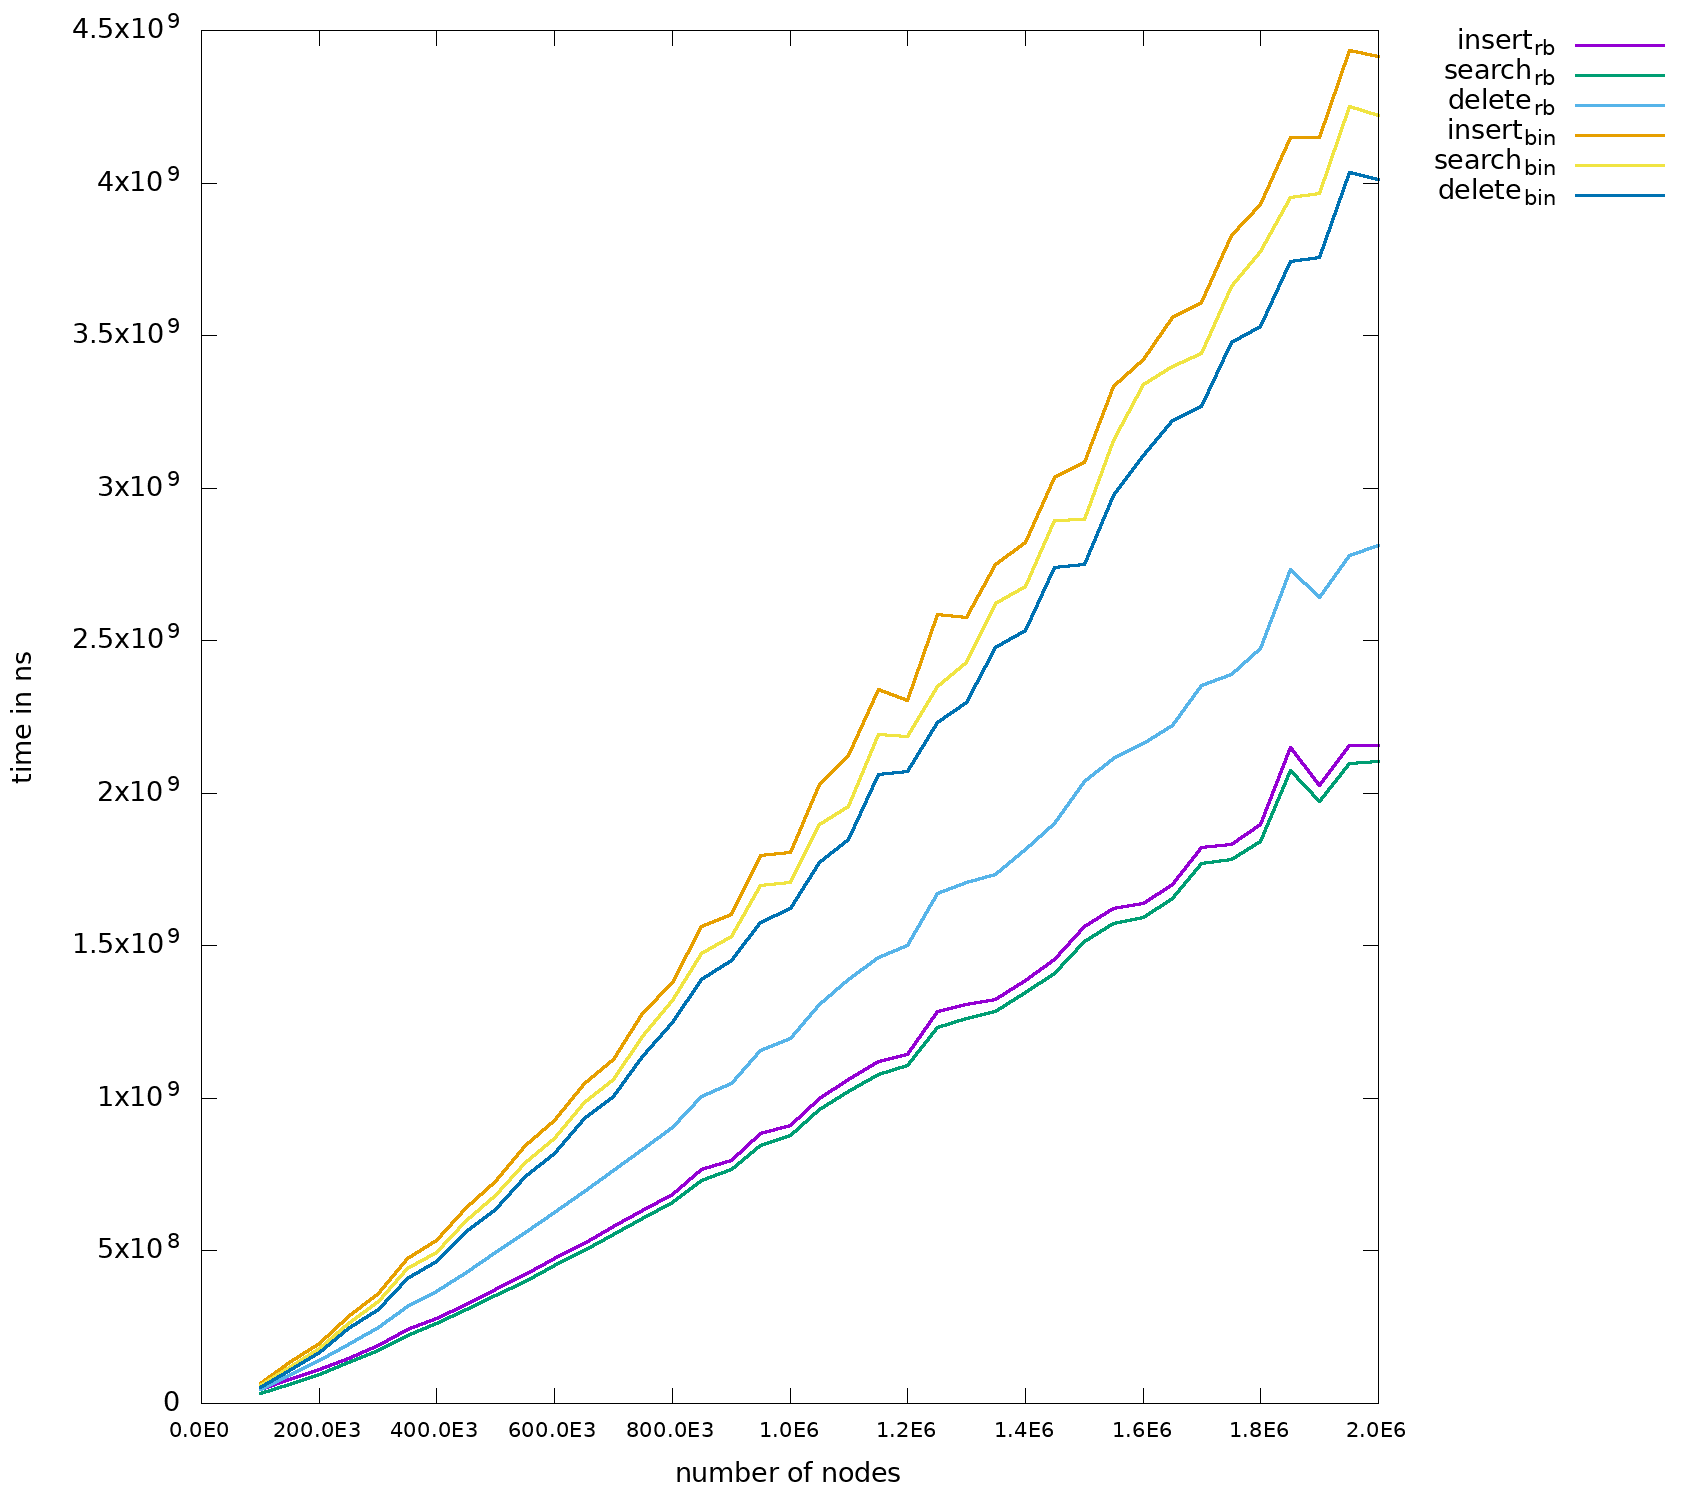
\includegraphics[width=200px]{../benchmark/compare_bin.png}
  \vspace{-20pt}
  \caption{Vergleich Laufzeit \gls{rbt}/\gls{bt}}
  \vspace{-15pt}
\end{wrapfigure}

Besonders wichtig ist es zu zeigen, dass unsere "Verbesserung" normalen Binary Trees tatsächlich performanter ist. In nebenstehender Abbildung kann man die Ergenisse des Benchmarks erkennen.
Die Graphen, die mit dem Index $_{rb}$ beschriftet sind, sind die des \gls{rbt} und die anderen gehören zum \gls{bt}.
Man kann erkenne, dass alle Operationen beim \gls{rbt} grundsätzlich schneller als die der Standardimplementierung sind. 
Der Unterschied zwischen den beiden Datenstrukturen ist nicht konstant sondern nimmt mit steigender Anzahl an Knoten immer weiter zu. 

Den Grund dafür kann man sehen, wenn man die Höhen der beiden Bäume vergleicht. Man kann sehen, dass sich der \gls{rbt} viel näher an der Höhe des vollständig balancierten Baumes befindet, 
als der \gls{bt}. Das sorgt dafür, dass man beim \gls{rbt} im Durchschnitt nicht so viele Vergleiche benötigt, bis man den Knoten erreicht, den man sucht oder einen \lstin{NULL}-Pointer, bei dem 
man einen neuen Knoten in den Baum einfügt. Das macht sich in den Benchmarks eindeutig bemerkbar.  

% TODO: pic heights

Eine weiter interessante Beobachtung ist, dass die Suche und die das Einfügen beim \gls{rbt} ungefähr gleich schnell sind, während das Löschen etwas langsamer als diese beiden Operationen ist.
Einen so starken Unterschied gibt es beim \gls{bt} nicht. Meine Hypothese dafür ist, dass das Rebalancieren beim Löschen von Knoten sehr viel langsamer ist, als das Rebalancieren beim Einfügen, weil
der Algorithmus häufig den ganzen Baum bis zur Wurzel durchgeht. 

\subsection{Recursive vs. Iterativ}

\begin{wrapfigure}{r}{200px}
  \centering
  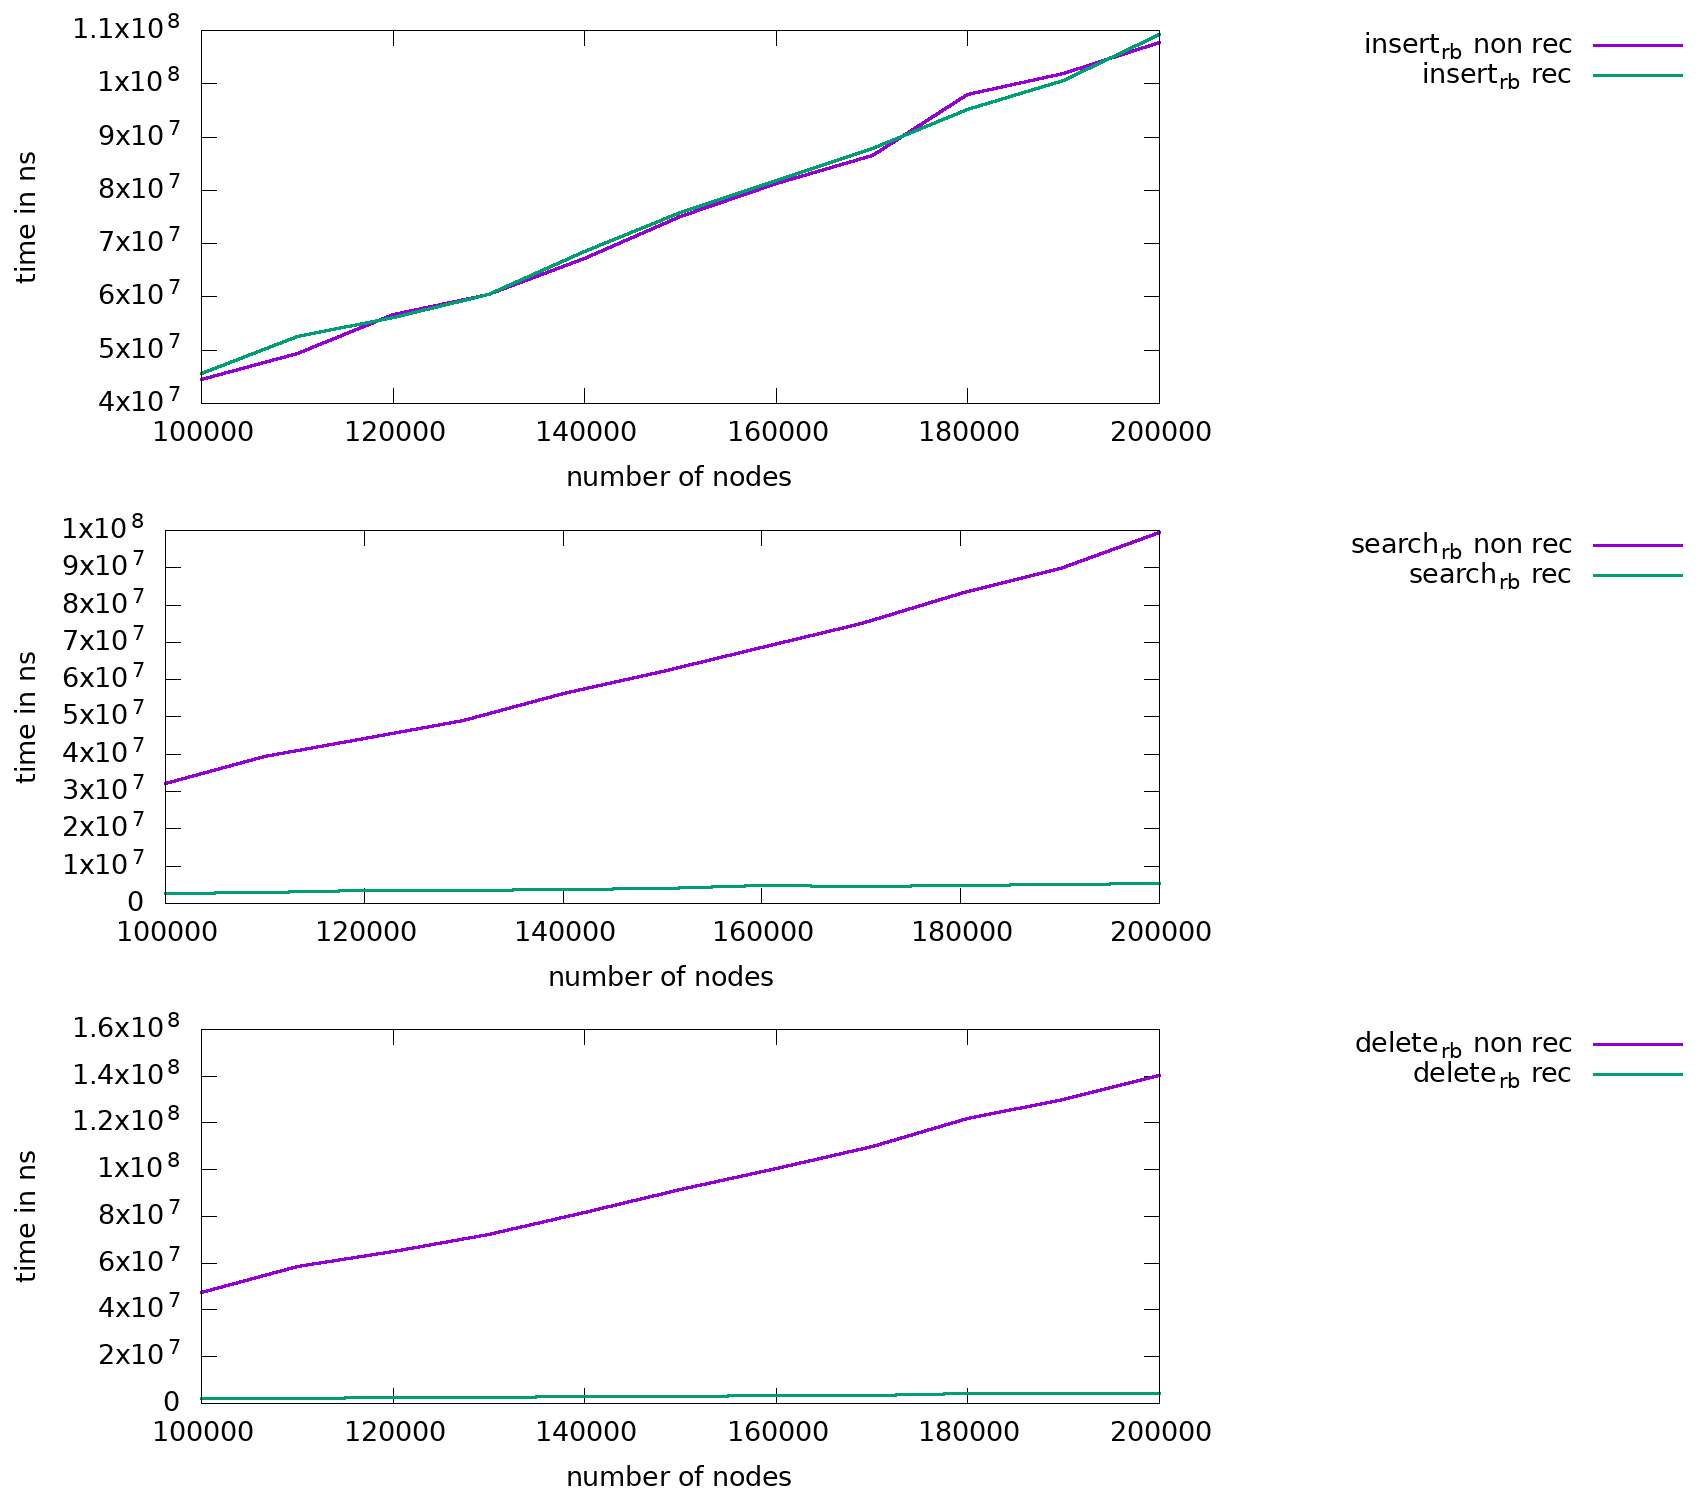
\includegraphics[width=200px]{../benchmark/compare_insert.png}
  \caption{Vergleich Rekursive/Iterative Implementierungen}
  \label{bir}
\end{wrapfigure}

Eine wichtige Frage, die sich während der Implementierung gestellt hat, ist, ob man die Operationen vom \gls{rbt} iterativ oder rekursiv implementiert. 
\gls{rec} wäre zwar die erste Sache, an die man dabei denkt, weil die Defintion von Bäumen auch meistens rekursiv ist. Außerdem werden meistens auch alle Algorithmen rekursiv beschrieben. 
Das Problem daran ist, dass durch sehr große Rekursionstiefe eventuell Leistungsprobleme entstehen können und teilweise auch sehr viel Speicher nötig ist. 
Deswegen wurde, wie schon in vorhergenden Kapiteln beschrieben, eine iterative und eine rekursive Version der \gls{dt} erstellt, um diese zu vergleichen.
Das Benchmark wurde wie in vorgehenden Abschnitt durchgeführt \ref{bbrbt} nur wurden hier die 2 verschiedenen Versionen der Programms getestet. 
Dafür wurde das Pythonscript verändert, sodass es zuerst die iterative Variante kompiliert und die Tests durchführt und in eine Datei schreibt und anschließend die Rekursive. 

Die Ergenisse sind in nachfolgenden Graphen in Abbildung \ref{bir} zu sehen. Es gibt jeweils einen Graph für die Suche, das Einfügen und das Löschen.

Man kann in allen drei Fällen erkennen, dass die iterative Variante (non rec) ab einer sehr großen Anzahl von Knoten konsistent schneller ist als die Rekursive (rec).
Meine Vermutung ist, dass es bei sehr großen Bäumen mit einer sehr großen Baumhöhe sehr viele Stackframes aufgebaut und auch wieder abgebaut werden müssen, wenn der rekursive Code ausgeführt wird.
Bei meiner anderen Implementierung gibt es einen Softwarestack, welcher nur die nötigen Daten speichert und sich auch nicht vergrößern muss, weil er schon mit der richtigen Größe erstellt wird.
Das könnte für den Signifikanten Unterschied in der Laufzeit der beiden Varianten führen.

\section{Speicher- und Zeitkomplexität} \label{time}

\section{Verwendung}

\begingroup
\parindent 0pt
\parskip 2ex
\def\enotesize{\normalsize}
\theendnotes
\endgroup

\bibliographystyle{alpha}
\bibliography{references} % see references.bib for bibliography management




\end{document}

% for citation:
% \cite{aad} for simple citation
% \cite[S. 20]{aad} for citation with page number(s)

% for acronyms and glossary ref:
% https://en.wikibooks.org/wiki/LaTeX/Glossary
% \gls{acro-name}

% Listings Example:
% \begin{lstlisting}[language=C]
%         #include <stdio.h>
%
%         int main(void)
%         {
%                 printf("Hello, World\n");
%                 return EXIT_SUCCESS;
%         }
% \end{lstlisting}

% TODO:
% Definitions
% Reference for Stackoverflow recursion depth in defs and traversal
% Pictures for tree and for tree array represantation


%\begin{minipage}{.5\textwidth}
%  \begin{center}
    \begin{tikzpicture} [
        inner sep = 0,
        level 1/.style = { sibling distance = 3cm },
        level 2/.style = { sibling distance = 1.5cm },
        every node/.style={draw, circle, minimum width = 1cm}
        ]
        
        \node {0}
        child [red, ->] { node [red, thick] {1} 
        child [blue] { node {3} } 
        child { node {5} } }
        child { node {200} 
        child { node {4} }
        child {node {200} } };
    \end{tikzpicture}
\end{center}  
%\end{minipage}
%\begin{minipage}{.4\textwidth}
%  \blindtext
%\end{minipage}